In the parametric sensitivity analysis reported in \cite{huff_key_2012}
\ref{sec:wfdeginv}, the results showed two regimes. In the first regime, the
mean of the peak annual dose rates is directly proportional to both the mass
factor (an inventory mass multiplier) and the fractional waste
form degradation rate. For some radionuclides, attenuation occurs for high
values of both parameters as the release of radionuclides is limited by
dispersion parameters. This phenomenon can be seen in the figures below in which
transition between regimes for higher degradation rates happens at lower mass
factors than transition between regimes for lower degradation rates.

The peaks for highly soluble, non-sorbing elements such as $I$ and $Cl$
are directly proportional to mass factor for most
values of waste form degradation rates. This effect can be seen in Figures
\ref{fig:WFDegI129} and \ref{fig:WFDegCl36}.


Highly soluble and non-sorbing $^{129}I$ demonstrates a direct proportionality between dose rate and
fractional degradation rate until a turnover where other natural system
parameters dampen transport.

\begin{figure}[ht!]
\begin{minipage}[b]{0.45\linewidth}
\centering
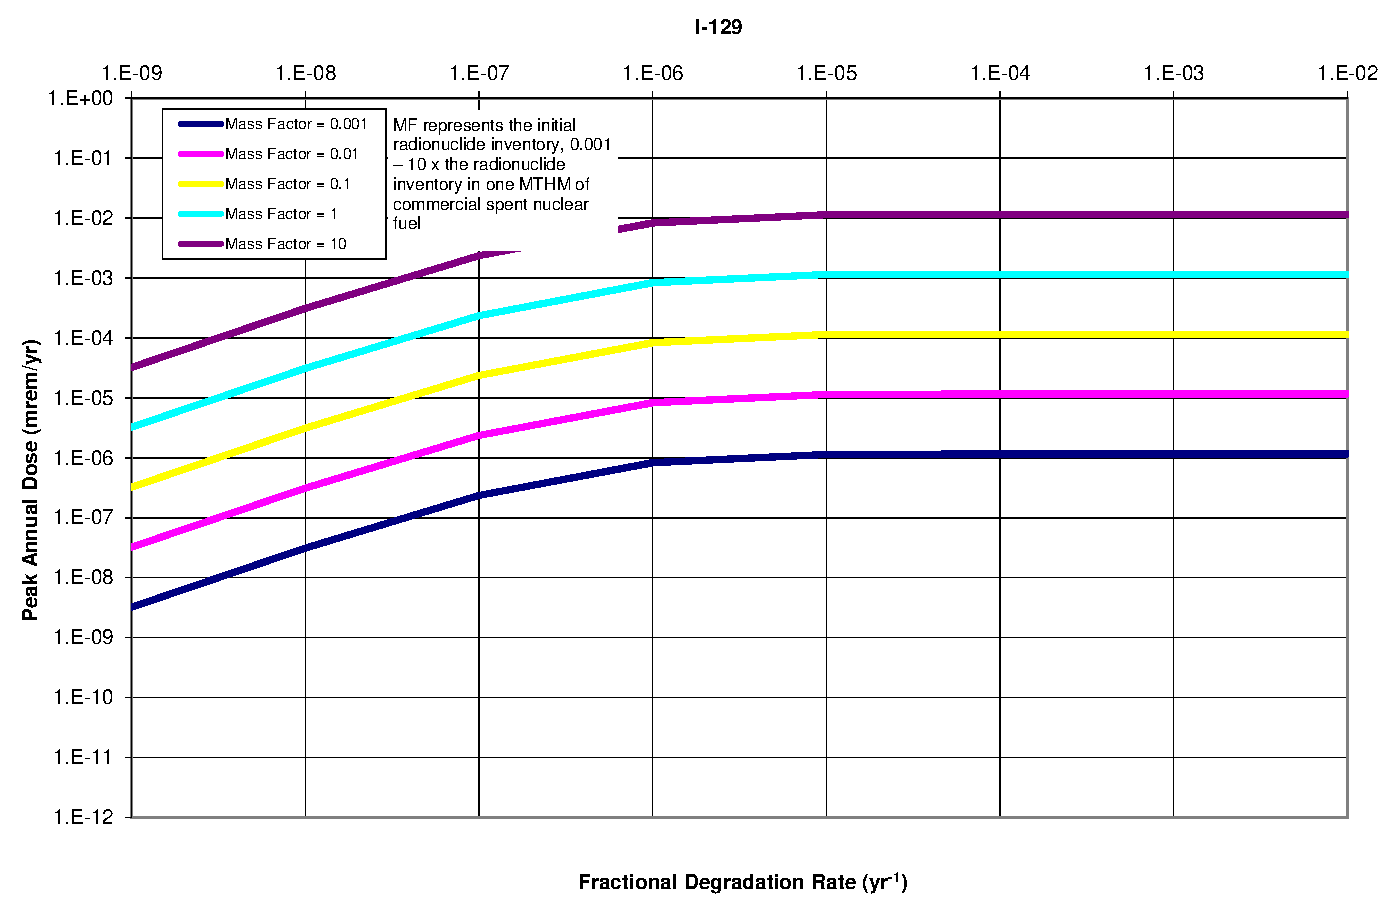
\includegraphics[width=\linewidth]{./results/images/WFDegAndInv/I-129.eps}
\caption{$^{129}I$ waste form degradation rate sensitivity.}
\label{fig:WFDegI129}

\end{minipage}
\hspace{0.05\linewidth}
\begin{minipage}[b]{0.45\linewidth}

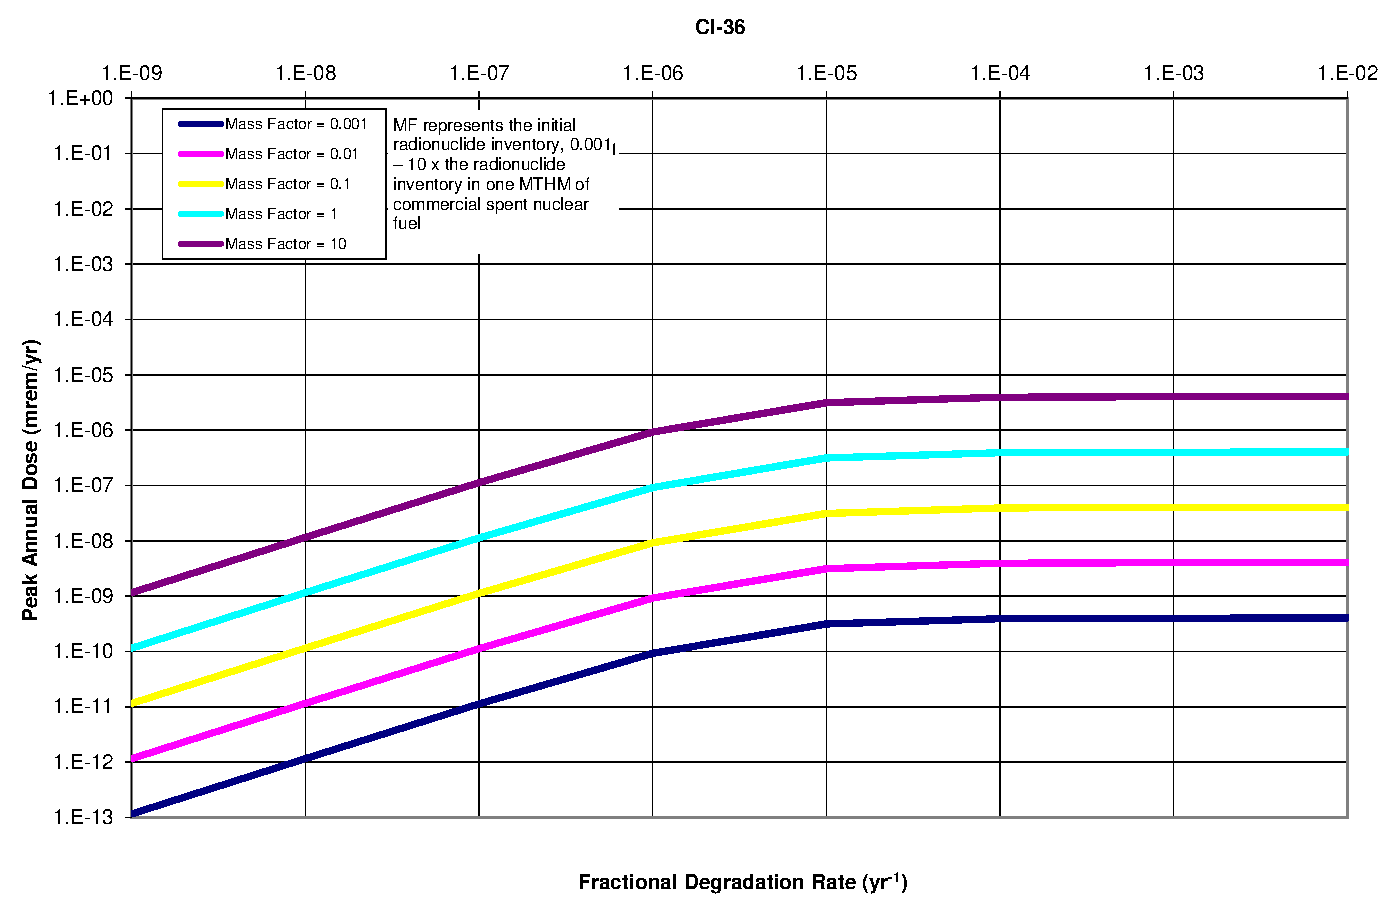
\includegraphics[width=\linewidth]{./results/images/WFDegAndInv/Cl-36.eps}
\caption{$^{36}Cl$ waste form degradation rate sensitivity.}
\label{fig:WFDegCl36}
\end{minipage}
\end{figure}

\FloatBarrier
